\documentclass{article}

\usepackage{fullpage}
\usepackage{color}
\usepackage{amsmath}
\usepackage{url}
\usepackage{verbatim}
\usepackage{graphicx}
\usepackage{parskip}
\usepackage{amssymb}
\usepackage{nicefrac}
\usepackage{listings} % For displaying code
\usepackage{graphicx}
\def\rubric#1{\gre{Rubric: \{#1\}}}{}

% Colors
\definecolor{blu}{rgb}{0,0,1}
\def\blu#1{{\color{blu}#1}}
\definecolor{gre}{rgb}{0,.5,0}
\def\gre#1{{\color{gre}#1}}
\definecolor{red}{rgb}{1,0,0}
\def\red#1{{\color{red}#1}}

% Math
\def\norm#1{\|#1\|}
\def\R{\mathbb{R}}
\def\argmax{\mathop{\rm arg\,max}}
\def\argmin{\mathop{\rm arg\,min}}
\newcommand{\mat}[1]{\begin{bmatrix}#1\end{bmatrix}}
\newcommand{\alignStar}[1]{\begin{align*}#1\end{align*}}

% LaTeX
\newcommand{\fig}[2]{\includegraphics[width=#1\textwidth]{a0f/#2}}
\newcommand{\centerfig}[2]{\begin{center}\includegraphics[width=#1\textwidth]{#2}\end{center}}
\def\items#1{\begin{itemize}#1\end{itemize}}
\def\enum#1{\begin{enumerate}#1\end{enumerate}}

\begin{document}

\title{CPSC 340 Assignment 0 (due 2018-01-10 at 9:00pm)}
% \author{Warm-up}
\date{}
\maketitle

\vspace{-4em}

\emph{Rationale for Assignment 0}: CPSC 340 is tough because it combines knowledge and skills across several disciplines. To succeed
in the course, you will need:
\begin{itemize}
\item Basic Python programming, including NumPy and plotting with matplotlib.
\item Math to the level of the course prerequisites: linear algebra, multivariable calculus, some probability.
\item Statistics, algorithms and data structures to the level of the course prerequisites.
\item Some basic LaTeX and git skills so that you can typeset equations and submit your assignments.
\end{itemize}

The purpose of this assignment is to make sure you are prepared for this course. I anticipate that each
of you will have different strengths and weaknesses, so don't be worried if you struggle with \emph{some} aspects
of the assignment. But if you find this assignment
to be very difficult overall, that is an early warning sign that you may not be prepared to take CPSC 340
at this time. Future assignments will be longer and more difficult than this one.


\section*{Instructions}
\rubric{mechanics:3}

\textbf{IMPORTANT!!!!! Before proceeding, please carefully read the general homework instructions at} \url{https://github.ugrad.cs.ubc.ca/CPSC340-2017W-T2/home/blob/master/homework_instructions.md}.
You need to be signed in to github.ugrad.cs.ubc.ca (using your CS ugrad id) in order to view this file.


\vspace{1em}
We use \blu{blue} to highlight the deliverables that you must answer/do/submit with the assignment.



\section{Linear Algebra Review}

For these questions you may find it helpful to review these notes on linear algebra:\\
\url{http://www.cs.ubc.ca/~schmidtm/Documents/2009_Notes_LinearAlgebra.pdf}

\subsection{Basic Operations}
\rubric{reasoning:7}

Use the definitions below,
\[
\alpha = 2,\quad
x = \left[\begin{array}{c}
0\\
1\\
2\\
\end{array}\right], \quad
y = \left[\begin{array}{c}
3\\
4\\
5\\
\end{array}\right],\quad
z = \left[\begin{array}{c}
1\\
2\\
-1\\
\end{array}\right],\quad
A = \left[\begin{array}{ccc}
3 & 2 & 2\\
1 & 3 & 1\\
1 & 1 & 3
\end{array}\right],
\]
and use $x_i$ to denote element $i$ of vector $x$.
\blu{Evaluate the following expresions} (you do not need to show your work).
\enum{
\item $\sum_{i=1}^n x_iy_i$ (inner product).
\item $\sum_{i=1}^n x_iz_i$ (inner product between orthogonal vectors).
\item $\alpha(x+y)$ (vector addition and scalar multiplication).
\item $\norm{x}$ (Euclidean norm of $x$).
\item $x^T$ (vector tranpose).
\item $A^T$ (matrix transpose).
\item $Ax$ (matrix-vector multiplication).
}
\textcolor{gre}{
Answer:
\enum{
\item $\sum_{i=1}^n x_iy_i=4+10=14$
\item $\sum_{i=1}^n x_iz_i=0$
\item $\alpha(x+y)=2*\left[\begin{array}{c}
3\\
5\\
7\\
\end{array}\right]=\left[\begin{array}{c}
6\\
10\\
14\\
\end{array}\right]$
\item $\norm{x}=\sqrt{1+4}=\sqrt{5}$
\item $x^T=\left[\begin{array}{ccc}
0&1&2\\
\end{array}\right]$
\item $A^T=\left[\begin{array}{ccc}
3&1&1\\
2&3&1\\
2&1&3\\
\end{array}\right]
$
\item  $Ax=\left[\begin{array}{c}
6\\
5\\
7\\
\end{array}\right]$
}
}
\subsection{Matrix Algebra Rules}
\rubric{reasoning:9}

Assume that $\{x,y,z\}$ are $n \times 1$ column vectors and $\{A,B,C\}$ are $n \times n$ real-valued matrices. \blu{State whether each of the below is true in general} (you do not need to show your work).

\begin{enumerate}
\item $x^Ty = \sum_{i=1}^n x_iy_i$.
\item $x^Tx = \norm{x}^2$.
\item $x^T(y+z) = z^Tx + x^Ty$.
\item $x^T(y^Tz) = (x^Ty)^Tz$.
\item $AB=BA$.
\item $A(B + C) = AB + AC$.
\item $(AB)^T = A^TB^T$.
\item $x^TAy = y^TA^Tx$.
\item $\det A \neq 0 \iff A$ is invertible.
\end{enumerate}
\textcolor{gre}{
Answer:
\enum{
\item True
\item True
\item True
\item False
\item False
\item True
\item False
\item True
\item True
}
}

\subsection{Special Matrices}
\rubric{reasoning:3}

\blu{In one sentence, write down the defining properties of the following special types of matrices}:
\enum{
\item Symmetric matrix.
\item Identity matrix.
\item Orthogonal matrix.
}
\textcolor{gre}{
Answer:
\enum{
\item A symmetric matrix is a square matrix $A$ that is equal to its transpose, $A=A^T$.
\item An identity matrix I of size n is a $n*n$ square matrix of which the values of main diagonal are 1 and values of others are 0.
\item An orthogonal matrix is a matrix $A$ of which the columns have the norm of 1 and with the property that $A^TA=I$
}
}
\section{Probability Review}


For these questions you may find it helpful to review these notes on probability:\\
\url{http://www.cs.ubc.ca/~schmidtm/Courses/340-F15/notes_probability.pdf}
And here are some slides giving visual representations of the ideas as well as some simple examples:\\
\url{http://www.cs.ubc.ca/~schmidtm/Courses/340-F17/probability.pdf}

\subsection{Rules of probability}
\rubric{reasoning:6}

\blu{Answer the following questions.} You do not need to show your work.

\begin{enumerate}
\item You flip 4 fair coins. What is the probability of observing \red{exactly} 3 heads?
\item You are offered the opportunity to play the following game: your opponent rolls 2 regular 6-sided dice. If the difference between the two rolls is at least 3, you win \$12. Otherwise, you get nothing. What is a fair price for a ticket to play this game once? In other words, what is the expected value of playing the game?
\item Consider two events $A$ and $B$ such that $\Pr(A, B)=0$. If $\Pr(A) = 0.4$ and $\Pr(A \cup B) = 0.95$, what is $\Pr(B)$? Note: $p(A, B)$ means
``probability of $A$ and $B$'' while $p(A \cup B)$ means ``probability of $A$ or $B$''. It may be helpful to draw a Venn diagram.
\end{enumerate}
\textcolor{gre}{
Answer:
\enum{
\item $P=\frac{{4 \choose 3}}{2^4}=\frac{4}{16}=\frac{1}{4}$
\item $price=12*\frac{(3+2+1)*2}{6*6}=4$
\item $Pr(B)=0.95-0.4=0.55$
}}
\subsection{Bayes Rule and Conditional Probability}
\rubric{reasoning:10}

\blu{Answer the following questions.} You do not need to show your work.

Suppose a drug test produces a positive result with probability $0.95$ for drug users, $P(T=1|D=1)=0.95$. It also produces a negative result with probability $0.99$ for non-drug users, $P(T=0|D=0)=0.99$. The probability that a random person uses the drug is $0.0001$, so $P(D=1)=0.0001$.

\begin{enumerate}
\item What is the probability that a random person would test positive, $P(T=1)$?
\item In the above, do most of these positive tests come from true positives or from false positives?
\item What is the probability that a random person who tests positive is a user, $P(D=1|T=1)$?
\item Are your answers from part 2 and part 3 consistent with each other?
\item What is one factor you could change to make this a more useful test?
\end{enumerate}
\textcolor{gre}{
Answer:
\enum{
\item $P(D=1)=0.0001\\P(D=0)=0.9999\\P(T=1)=0.95*0.0001+0.9999*(1-0.99)=0.010094$
\item true positives$=0.95*0.0001=0.000095$\\false positive$=0.9999*0.01=0.009999>0.000095$\\so false positive
\item $P(D=1|T=1)=P(D=1)/P(T=1)=0.0001/0.010094\approx0.0099$
\item Yes. In positive tests, only about 0.0099 are drug users. This means the majority is not drug users which is the same as the false positive.
\item From the equation that $P(T=1)=P(D=1)P(T=1|D=1)+P(D=0)P(T=1|D=0)$, if we want true positive does the most, we have to decrease $P(T=1|D=0)$ or increase $P(D=1)$
}}

\section{Calculus Review}


\subsection{One-variable derivatives}
\rubric{reasoning:8}

\blu{Answer the following questions.} You do not need to show your work.

\begin{enumerate}
\item Find the minimum value of the function $f(x) = 3x^2 -2x + 5$ for $x \in \R$.
\item Find the maximum value of the function $f(x) = x(1-x)$ for $x$ in the interval $[0,1]$.
\item Find the minimum value of the function $f(x) = x(1-x)$ for $x$ in the interval $[0,1]$.
\item Let $p(x) = \frac{1}{1+\exp(-x)}$ for $x \in \R$. Compute the derivative of the function $f(x) = -\log(p(x))$ and simplify it by using the function $p(x)$.
\end{enumerate}
Remember that in this course we will $\log(x)$ to mean the ``natural'' logarithm of $x$, so that $\log(\exp(1)) = 1$. Also, obseve that $p(x) = 1-p(-x)$ for the final part.
\textcolor{gre}{
\enum{
\item $f'(x)=6x-2=0\\x=\frac{1}{3}\\f''(x)=6>0\\$so we can get minimum at $x=\frac{1}{3}\\f(\frac{1}{3})=\frac{14}{3}$
\item $f'(x)=-2x+1=0\\x=\frac{1}{2}\\f''(x)=-2<0\\$so we can get maximum at $\frac{1}{2}\\f(\frac{1}{2})=\frac{1}{4}$
\item The same as above for $f'(x),f''(x)$. To get the minimum value, we have to compare f(0)=0 and f(1)=0. So we can get minimum at 0 and 1, and the minimum value is 0.
\item $f(x)=log(1+e^{-x})\\f'(x)=-\frac{e^{-x}}{1+e^{-x}}=-1+\frac{1}{1+e^{-x}}=-1+p(x)$
}}
\subsection{Multi-variable derivatives}
\rubric{reasoning:5}

\blu{Compute the gradient $\nabla f(x)$ of each of the following functions.} \red{You do not need to show your work.}
\begin{enumerate}
\item $f(x) = x_1^2 + \exp(x_2)$ where $x \in \R^2$.
\item $f(x) = \exp(x_1 + x_2x_3)$ where $x \in \mathbb{R}^3$.
\item $f(x) = a^Tx$ where $x \in \R^2$ and $a \in \R^2$.
\item $f(x) = x^\top A x$ where $A=\left[ \begin{array}{cc}
2 & -1 \\
 -1 & 1 \end{array} \right]$ and $x \in \mathbb{R}^2$.
 \item $f(x) = \frac{1}{2}\norm{x}^2$ where $x \in \R^d$.
\end{enumerate}

Hint: it is helpful to write out the linear algebra expressions in terms of summations.
\textcolor{gre}{
Answer:
\enum{
\item  $\bigtriangledown f(x)=\left[\begin{array}{c}
2x_1\\
exp(x_2)\\
\end{array}\right]$
\item  $\bigtriangledown f(x)=\left[\begin{array}{c}
exp(x_1+x_2x_3)\\
x_3exp(x_1+x_2x_3)\\
x_2exp(x_1+x_2x_3)\\
\end{array}\right]$
\item $\bigtriangledown f(x)=\alpha$
\item  $\bigtriangledown f(x)=\left[\begin{array}{c}
4x_1-2x_2\\
2x_2-2x_1\\
\end{array}\right]$
\item $\bigtriangledown f(x)=x$
}
}



\subsection{Derivatives of code}

\rubric{code:4}

Note: for info on installing and using Python, see \url{https://github.ugrad.cs.ubc.ca/CPSC340-2017W-T2/home/blob/master/python_info.md}.

Your repository contains a file named \texttt{grads.py} which defines several Python functions that take in an input variable $x$, which we assume to be a 1-d array (in math terms, a vector).
It also includes (blank) functions that return the corresponding gradients.
For each function, \blu{write code that computes the gradient of the function} in Python.
You can do this directly in \texttt{grads.py}; no need to make a fresh copy of the file. However, per the homework instructions, you should add a link to your README file so that the TA can access it easily.

Hint: it's probably easiest to first understand on paper what the code is doing, then compute
the gradient, and then translate this gradient back into code.

Note: do not worry about the distinction between row vectors and column vectors here.
For example, if the correct answer is a vector of length 5, we'll accept numpy arrays
of shape \texttt{(5,)} (a 1-d array) or \texttt{(5,1)} (a column vector) or
\texttt{(1,5)} (a row vector). In future assignments we will start to be more careful
about this.

Warning: Python uses whitespace instead of curly braces to delimit blocks of code.
Some people use tabs and other people use spaces. My text editor (Atom) inserts 4 spaces (rather than tabs) when
I press the Tab key, so the file \texttt{grads.py} is indented in this manner. If your text editor inserts tabs,
Python will complain and you might get mysterious errors... this is one of the most annoying aspects
of Python, especially when starting out. So, please be aware of this issue! And if in doubt you can just manually
indent with 4 spaces, or convert everything to tabs. For more information
see \url{https://www.youtube.com/watch?v=SsoOG6ZeyUI}.
\textcolor{gre}{
Answer:\\
%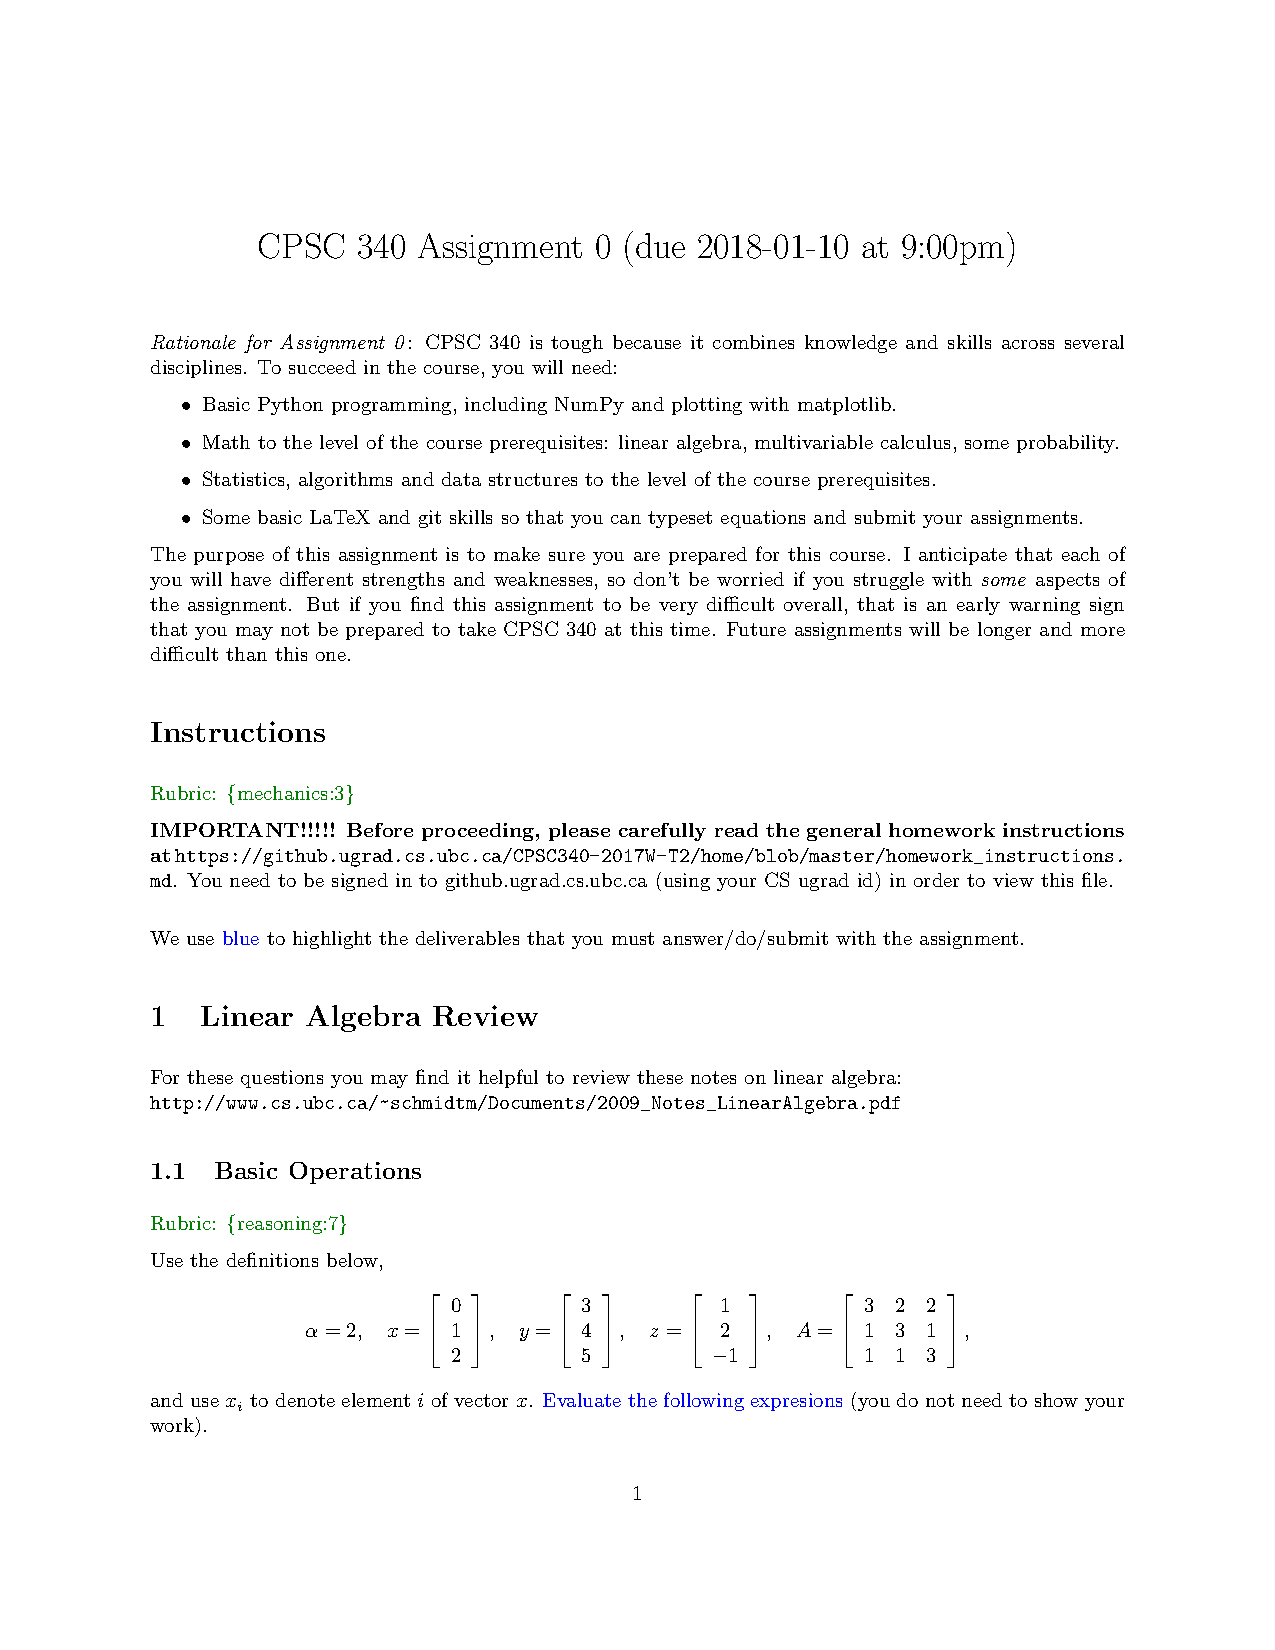
\includegraphics[height=5cm]{a0.png}\\
The code of the solution is in \url{https://github.ugrad.cs.ubc.ca/CPSC340-2017W-T2/u7p1b_a0/blob/master/code/grads.py}
}
\section{Algorithms and Data Structures Review}

\subsection{Trees}
\rubric{reasoning:2}

\blu{Answer the following questions.} You do not need to show your work.

\begin{enumerate}
\item What is the maximum number of \emph{leaves} you could have in a binary tree of depth $l$?
\item What is the maximum number of \emph{nodes} (including leaves) you could have in a binary tree of depth $l$?
\end{enumerate}
Note: we'll use the convention that the leaves are not included in the depth, so for $l=1$ the answers would be 2 and 3 respectively.
\textcolor{gre}{
Answer:
\enum{
\item $2^l$
\item $2^{l+1}-1$
}}
\subsection{Common Runtimes}
\rubric{reasoning:4}

\blu{Answer the following questions using big-$O$ notation} You do not need to show your work.
\begin{enumerate}
\item What is the cost of running the mergesort algorithm to sort  a list of $n$ numbers?
\item What is the cost of finding the third-largest element of an unsorted list of $n$ numbers?
\item What is the cost of finding the smallest element greater than 0 in a \emph{sorted} list with $n$ numbers.
\item What is the cost of computing the matrix-vector product $Ax$ when $A$ is $n \times d$ and $x$ is $d \times 1$.
\end{enumerate}
\textcolor{gre}{
Answer:
\enum{
\item $O(nlog(n))$
\item $O(n)$
\item $O(log(n))$
\item $O(nd)$
}}
\subsection{Running times of code}
\rubric{reasoning:4}

Your repository contains a file named \texttt{bigO.py}, which defines several functions
that take an integer argument $N$. For each function, \blu{state the running time as a function of $N$, using big-O notation}.
Please include your answers in your report. Do not write your answers inside \texttt{bigO.py}.
\textcolor{gre}{
Answer:
\enum{
\item $O(N)$
\item $O(N)$
\item $O(1)$
\item $O(N^2)$
}}
\vspace{50pt}
\underline{\emph{ARE YOU SURE YOU'RE FOLLOWING ALL THE HOMEWORK SUBMISSION INSTRUCTIONS?}}



\end{document}
